\documentclass[a4paper, 10pt]{article}%тип документа

%отступы
\usepackage[left=2cm,right=2cm,top=2cm,bottom=3cm,bindingoffset=0cm]{geometry}

%Русский язык
\usepackage[T2A]{fontenc} %кодировка
\usepackage[utf8]{inputenc} %кодировка исходного кода
\usepackage[english,russian]{babel} %локализация и переносы

%Вставка картинок
\usepackage{graphicx}
\graphicspath{{pictures/}}
\DeclareGraphicsExtensions{.pdf,.png,.jpg}

%Графики
\usepackage{pgfplots}
\pgfplotsset{compat=1.9}

%Математика
\usepackage{amsmath, amsfonts, amssymb, amsthm, mathtools}

%Заголовок
\author{Валеев Рауф Раушанович \\
группа 825}
\title{Работа 1.3.1 \\
Определение модуля Юнга на основе исследования деформаций растяжения и изгиба}
\begin{document}
\maketitle
\newpage
\textbf{Цель работы:} экспериментально получить зависимость между напряжением и деформацией (закон Гука) для двух простейших напряженных состояний упругих тел: одноосного растяжения и чистого изгиба; по результатам измерений вычислить модуль Юнга. \\
\textbf{В работе используется:} прибор лермантова, проволока из исследуемого материала, зрительная трубка со шкалой, набор грузов, микрометр, рулетка; во второй части - стойка для изгибания балки, индикатор для измерения величины прогиба, набор исследуемых стержней, грузы, линейка, штангенциркуль.
\center{\textbf{Определение модуля Юнга по измерениям растяжения проволоки (рис.1)}}
\begin{figure}[h]
\center{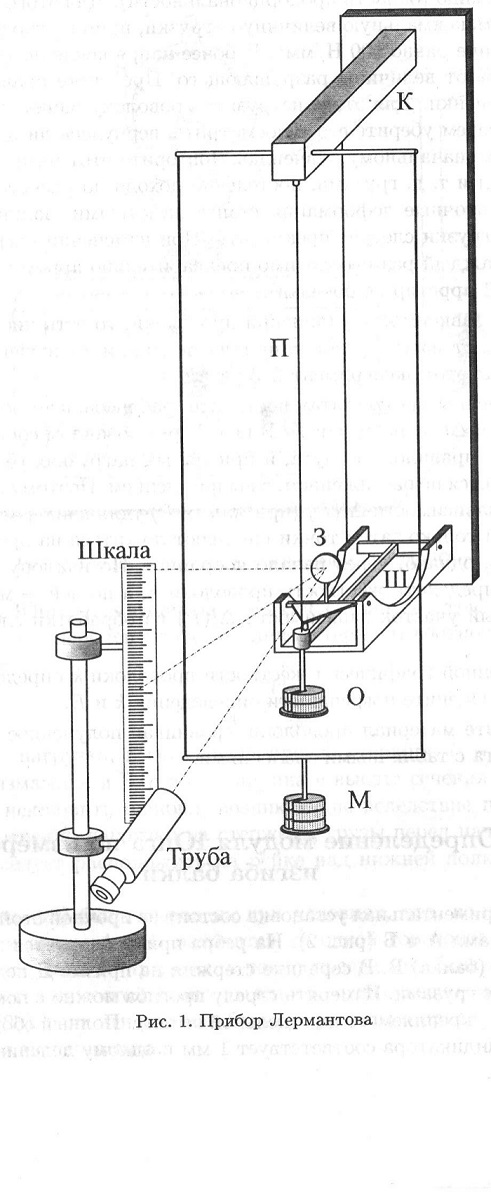
\includegraphics{131_1.jpg}}
\end{figure}
\begin{enumerate}
\item $d = (0,46 \pm 0,01) \text{см}$.
\item Измеряем площадь поперечного сечения проволоки
\[S =\dfrac{ \pi (\overline{d})^2}{4} = 0,166 \text{ см}^2\]
\[\sigma_S = S\sqrt{2\left( \dfrac{\sigma_d}{d}\right) ^2} = 0,005 \text{ см}^2\]
\[S = (0,166\pm0,005) \text{ мм}^2\]
\item Измеряем длинну проволоки $l = 176  \text{ см}$
\item Направляем зрительную трубу на зеркальце так, чтобы мы четко видели шкалу, тогда свет от шкалы будет падать примерно перпендикулярно шкале на зеркало, поэтому
\[\Delta l =\dfrac{nr}{2h}\]
\[ \sigma_{\Delta l} = \Delta l\sqrt{\left( \dfrac{\sigma_{n}}{n}\right)^2 + \left(\dfrac{\sigma_d}{d}\right)^2+\left(\dfrac{\sigma_h}{h}\right)^2} \]
где $r = 15$ см - длина рычага, разница показаний шкалы - $n$, расстояние от шкалы до проволоки - $h = (138\pm0,1)\text{ см}$.
\item Исходя из того, что $\sigma_{\text{предел}} = 900 \text{ Н}/\text{мм}^2$ получаем, что предельный вес, который можно повесить, чтобы не выйти за пределы $P_{\text{предел}} = 0,3 \sigma_{\text{предел}} S \approx 44,8 H$. 
\item Снимем зависимость удлинения проволоки от массы грузов при увеличении и уменьшении нагрузки 2-3 раза (табл.1). 
\item Построим график зависимости удлинения проволоки от нагрузки. В недеформированном состоянии проволока, как правило, изогнута, и при малых нагрузках её "удлинение" определяется не растяжением, а выпрямлением. Найдем уравнение получившийся прямой по МНК. По наклону прямой определим жесткость проволоки, а по ней - модуль Юнга (табл.2). Начальный участок графика при обработке следует исключить. 
\item По найденной графически жёсткости проволоки найдем модуль Юнга по формуле
\[E = \dfrac{k*l_0}{S}\]
\[\sigma_E = \sqrt{\left( \dfrac{\sigma_{k}}{k} \right)^2 + \left( \dfrac{\sigma_{S}}{S} \right)^2 + \left( \dfrac{\sigma_{l_0}}{l_0} \right)^2 }\]
\end{enumerate}

\begin{tikzpicture}
\begin{axis} [title = Зависимость удлинения проволоки от нагрузки,
		xlabel=$\Delta l \text{, мм}$,
		ylabel= {P, Н}]
\addplot coordinates {
(0.326, 9.48)
(0.331, 9.48)
(0.315, 9.48)
(0.342, 9.48)
(0.326, 9.48)
(0.337, 9.48)
(0.641, 14.41)
(0.63, 14.41)
(0.614, 14.41)
(0.63, 14.41)
(0.641, 14.41)
(0.897, 18.87)
(0.886, 18.87)
(0.88, 18.87)
(0.902, 18.87)
(0.886, 18.87)
(0.870, 18.87)
(1.168, 23.6)
(1.152, 23.6)
(1.158, 23.6)
(1.163, 23.6)
(1.152, 23.6)
(1.152, 23.6)
(1.44, 28.53)
(1.429, 28.53)
};
\addplot coordinates {
(0, 3.61)
(1.5, 29.56)
};
\end{axis}
\end{tikzpicture}
\newpage
\center{\textbf{Определение модуля Юнга по измерениям изгиба палки (рис.2)}}
\begin{figure}[h]
\center{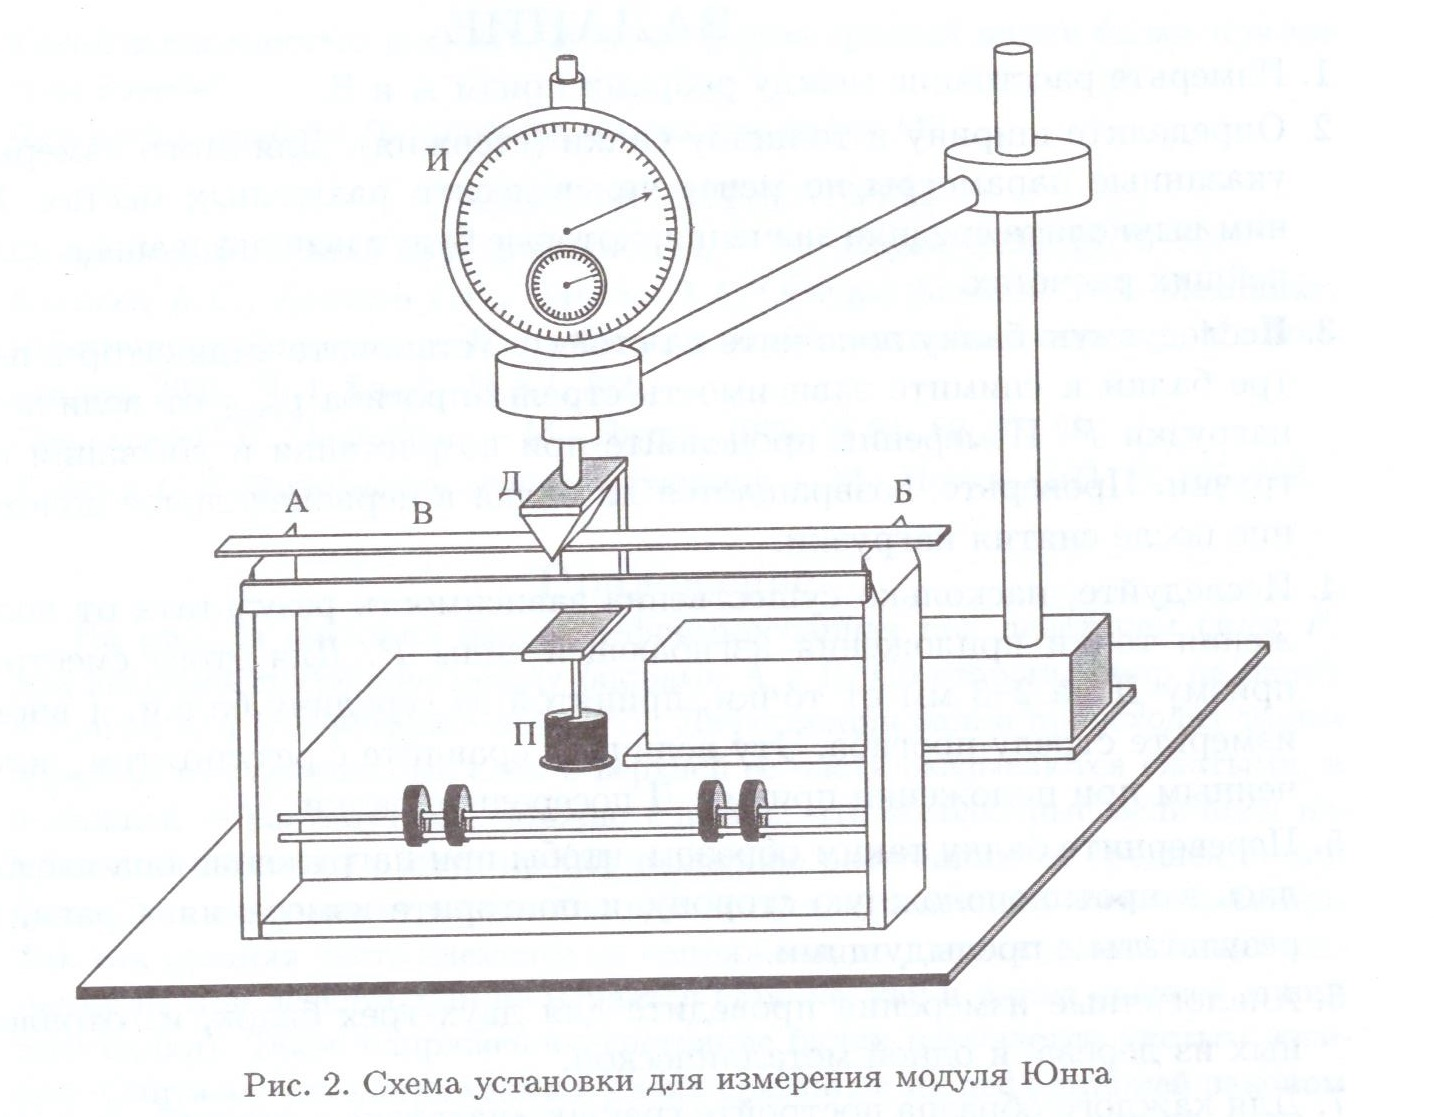
\includegraphics{131_2.jpg}}
\end{figure}
\begin{enumerate}
\item Измеряем $l_{ab} = 50$ см.
\item Определяем ширину и толщину стержней (табл. 3). 
\item Кладем балку так, чтобы Д было в середине и снимаем зависимость $y_{max}$ от P. Для этого смещаем Д на 2-3 мм в сторону и сравниваем с положением в середине: угол наклона примерно один и тот же.
\item Поворачиваем балку на 180 градусов вокруг горизонтальной оси и проделываем то же, что и в пункте 3. Сравниваем с пунктом 3:  угол наклона примерно один и тот же.  
\item Аналогично для 2-3 балок из дерева и 1 из метала. 
\item Все данные записываем в табл. 4. 
\item Для каждого образца строим графики при увеличении и уменьшении нагрузки.
\item По наклону графиков определяем средние значения модулей Юнга по формуле (табл.5)
\[E = \dfrac{Pl^3}{4ab^3y_{max}}\]
\[\sigma_E = \sqrt{3 \left( \dfrac{\sigma_{l}}{l} \right)^2 + \left( \dfrac{\sigma_{P/y_{max}}}{P/y_{max}} \right)^2 + \left( \dfrac{\sigma_{a}}{a} \right)^2 + 3 \left( \dfrac{\sigma_{b}}{b} \right)^2}\]
\end{enumerate}
\begin{tikzpicture}
\begin{axis} [title = График табл.4,
		xlabel=$y_{max} \text{, мм}$,
		ylabel= {P, Н}]
\addplot coordinates {
(0.67, 4.973)
(0.7, 4.973)
(0.69, 4.973)
(0.71, 4.973)
(0.58, 4.973)
(0.63, 4.973)
(0.76, 4.973)
(0.68, 4.973)
(1.28, 9.521)
(1.31, 9.521)
(1.21, 9.521)
(1.24, 9.521)
(1.33, 9.521)
(1.38, 9.521)
(1.31, 9.696)
(1.33, 9.696)
(1.91, 14.197)
(1.94, 14.244)
(1.92, 14.244)
(1.94, 14.241)
(1.93, 14.241)
(1.94, 14.244)
(1.97, 14.244)
(1.97, 14.197)
(2.51, 18.92)
(2.55, 18.92)
(2.58, 18.92)
(2.6, 18.92)
(2.52, 18.92)
(2.58, 18.92)
(2.55, 18.92)
(2.54, 18.92)
};
\addplot coordinates {
(0, -0.003)
(2.7, 19.96)
};
\end{axis}
\end{tikzpicture}

\begin{tikzpicture}
\begin{axis} [
		xlabel=$y_{max} \text{, мм}$,
		ylabel= {P, Н}]
\addplot coordinates {
(0.69, 4.973)
(0.72, 4.973)
(0.68, 4.973)
(0.7, 4.973)
(1.42, 9.519)
(1.4, 9.519)
(1.39, 9.519)
(1.45, 9.519)
(2.12, 14.244)
(2.11, 14.244)
(2.09, 14.246)
(2.13, 14.244)
(2.78, 18.92)
(2.8, 18.92)
(2.82, 18.92)
(2.81, 18.92)
};
\addplot coordinates {
(0, 0.3)
(3, 20)
};
\end{axis}
\end{tikzpicture}

\begin{tikzpicture}
\begin{axis} [
		xlabel=$y_{max} \text{, мм}$,
		ylabel= {P, Н}]
\addplot coordinates {
(0.71, 4.973)
(0.65, 4.973)
(0.74, 4.973)
(0.75, 4.973)
(1.37, 9.519)
(1.34, 9.519)
(1.43, 9.519)
(1.4, 9.519)
(2.06, 14.244)
(2.03, 14.244)
(2.06, 14.244)
(2.08, 14.244)
(2.73, 18.92)
(2.74, 18.92)
(2.75, 18.92)
(2.76, 18.92)
};
\addplot coordinates {
(0, -0.003)
(3, 20.6)
};
\end{axis}
\end{tikzpicture}

\newpage
\begin{table}
\center{
\begin{tabular}{|c|c|c|c|c|c||c|c|c|c|c|}
\hline
P, Н & 9,48 &14,41 &18,87&23,60 &28,53 &28,53 &23,60 &18,87 &14,41 &9,48\\
\hline
$\Delta l$, см&0,326 &0,641 &0,897 &1,168 &1,440 &1,440 &1,163 &0,902 &0,641 &0,342\\ 
\hline
$\sigma_{\Delta l}$&0,007 &0,014 &0,020 &0,025 &0,031 &0,031 &0,025 &0,020 &0,014 &0,008\\
\hline
\hline
P, Н & 9,48 &14,41 &18,87&23,60 &28,53 &28,53 &23,60 &18,87 &14,41 &9,48\\
\hline
$\Delta l$, см&0,331 &0,630 &0,886 &1,152 &1,429 &1,429 &1,152 &0,886 &0,630 &0,326\\
\hline
$\sigma_{\Delta l}$&0,007 &0,014 &0,019 &0,025 &0,031 &0,031 &0,025 &0,019 &0,014 &0,007\\
\hline
\hline
P, Н & 9,48 &14,41 &18,87&23,60 &28,53 &28,53 &23,60 &18,87 &14,41 &9,48\\
\hline
$\Delta l$&0,315 &0,630 &0,880 &1,158 &1,429 &1,424 &1,152 &0,870 &0,614 &0,337\\
\hline
$\sigma_{\Delta l}$&0,007 &0,014 &0,019 &0,025 &0,031 &0,031 &0,025 &0,019 &0,013 &0,008\\
\hline
\end{tabular}
}
\caption{Зависимость удлинения проволоки от нагрузки}
\center{
\begin{tabular}{|c|c|c|c|}
\hline
&Значение&$\sigma$&$\varepsilon$\\
\hline
k&$1,73*10^3$ H/м&$0,027*10^3$ Н/м&0,016\\
\hline
E&$18,3*10^{10}$ Па&$ 0,7*10^{10}$ Па&0,04\\
\hline
\end{tabular}
}
\caption{Значения k и E}
\begin{tabular}{|c|c|c|c|c|c|c|c|c|c|c|c|c|}
\hline
&1&2&3&4&5&6&7&8&9&10&Ср.знач.&$\sigma$\\
\hline
\multicolumn{13}{|c|}{1 балка}\\
\hline
a, см&0,4&0,4&0,39&0,38&0,35&0,37&0,38&0,39&0,38&0,37&0,381&0,01\\
\hline
b, см&2,1&2,1&2,12&2,12&2,09&2,09&2,07&2,12&2,08&2,08&2,097&0,01\\
\hline
\multicolumn{13}{|c|}{2 балка}\\
\hline
a, см&0,46&0,51&0,41&0,46&0,46&0,46&0,47&0,48&0,46&0,47&0,464&0,01\\
\hline
b, см&2,15&2,14&2,15&2,15&2,12&2,15&2,15&2,14&2,14&2,15&2,144
&0,01\\
\hline
\multicolumn{13}{|c|}{3 балка}\\
\hline
a, см&0,95&0,94&0,94&0,93&0,92&0,95&0,94&0,92&0,93&0,92&0,934&0,004\\
\hline
b, см&2,02&2,07&2,04&2,02&2,02&2&2&2,02&2,01&2,04&2,024&0,006\\
\hline
\end{tabular}
\caption{Значения a и b}
\end{table}
\newpage
\begin{table}
\center{
\begin{tabular}{|c|c|c|c|c||c|c|c|c|}
\hline
\multicolumn{9}{|c|}{Сталь, несмещенная}\\
\hline
P, H&4,973&9,521&14,197&18,92&18,92&14,197&9,521&4,973\\
\hline
$y_{max}$, мм&0,67&1,28&1,91&2,51&2,6&1,97&1,38&0,76\\
\hline
\multicolumn{9}{|c|}{Сталь, несмещенная, перевернутая}\\
\hline
P, H&4,973&9,521&14,244&18,92&18,92&14,244&9,521&4,973\\
\hline
$y_{max}$, мм&0,63&1,24&1,94&2,52&2,58&1,97&1,33&0,7\\
\hline
\multicolumn{9}{|c|}{Сталь, смещенная}\\
\hline
P, H&4,973&9,696&14,241&18,92&18,92&14,241&9,696&4,973\\
\hline
$y_{max}$, мм&0,69&1,31&1,93&2,55&2,54&1,94&1,33&0,71\\
\hline
\multicolumn{9}{|c|}{Сталь, смещенная, перевернутая}\\
\hline
P, H&4,973&9,521&14,244&18,92&18,92&14,244&9,521&4,973\\
\hline
$y_{max}$, мм&0,58&1,21&1,92&2,55&2,58&1,94&1,31&0,68\\
\hline
\multicolumn{9}{|c|}{Латунь}\\
\hline
P, H&4,973&9,519&14,244&18,92&18,92&14,244&9,519&4,973\\
\hline
$y_{max}$, мм&0,69&1,42&2,09&2,78&2,82&2,11&1,39&0,7\\
\hline
\multicolumn{9}{|c|}{Латунь, перевернутая}\\
\hline
P, H&4,973&9,519&14,244&18,92&18,92&14,244&9,519&4,973\\
\hline
$y_{max}$, мм&0,72&1,4&2,13&2,8&2,81&2,12&1,45&0,72\\
\hline
\multicolumn{9}{|c|}{Дерево}\\
\hline
P, H&4,973&9,519&14,244&18,92&18,92&14,244&9,519&4,973\\
\hline
$y_{max}$, мм&0,71&1,37&2,06&2,73&2,74&2,08&1,43&0,74\\
\hline
\multicolumn{9}{|c|}{Дерево, перевернутая}\\
\hline
P, H&4,973&9,519&14,244&18,92&18,92&14,244&9,519&4,973\\
\hline
$y_{max}$, мм&0,65&1,34&2,03&2,75&2,76&2,06&1,4&0,75\\
\hline
\end{tabular}
}
\caption{Зависимость P от $y_{max}$ для разных балок в разном положении}
\end{table}
\begin{table}
\center{
\begin{tabular}{|c|c|c|c|}
\hline
\multicolumn{4}{|c|}{1 балка}\\
\hline
&Значение&$\sigma$&$\varepsilon$\\
\hline
$P/y_{max}$&7393,58 Н/м&74,53 Н/м&0,01\\
\hline
E&$20,05*10^{10}$ Н/м& $0,03*10^{10}$ Н/м&0,014\\
\hline
\end{tabular}
\begin{tabular}{|c|c|c|c|}
\hline
\multicolumn{4}{|c|}{2 балка}\\
\hline
&Значение&$\sigma$&$\varepsilon$\\
\hline
$P/y_{max}$&6665,41 Н/м&41,89 Н/м&0,01\\
\hline
E&$9,72*10^{10}$ Н/м& $0,464*10^{10}$ Н/м&0,048\\
\hline
\end{tabular}
\begin{tabular}{|c|c|c|c|}
\hline
\multicolumn{4}{|c|}{3 балка}\\
\hline
&Значение&$\sigma$&$\varepsilon$\\
\hline
$P/y_{max}$&6868,97 Н/м&64,24 Н/м&0,01\\
\hline
E&$1,31*10^{10}$ Н/м& $0.0221*10^{10}$ Н/м&0,017\\
\hline
\end{tabular}
}
\caption{Вычисляемые значения для балок}
\end{table}
\end{document}